\chapter{Introduction}

The Standard Model (SM) of particle physics continues to be one of mankind's 
greatest intellectual achievements. With the discovery of the Higgs boson at the
Large Hadron Collider in 2012 by both the ATLAS and CMS experiments
\cite{Aad:2012tfa, Chatrchyan:2012xdj}, all particles predicted by the SM have
been observed.  However, there remains many outstanding issues which the SM
fails to explain.  One such issue is the composition and nature of dark matter
(DM).




The existence of additional $U(1)$ gauge symmetries of nature are common in
several Beyond the Standard Model (BSM) theories 
\cite{Goodsell:2010ie, Abel:2008ai, Candelas:1985en, Andreas:2011in, Jaeckel:2010ni}.
Such theories envision the associated gauge boson ($A'$, ``dark'', ``hidden'',
``heavy'' photon) inhabiting a  ``hidden sector'' consisting of a complex of 
particles and gauge bosons.  Probing the structure of such a hidden sector may
be possible through the so called ``Vector'' portal which describes  
the weak coupling of the $A'$ to charged particles through ``kinetic mixing''
with the photon. In fact, it is natural for the $A'$ to 
kinetically mix with the Standard Model (SM) photon through the interaction
of massive fields carrying both SM hypercharge and dark charge \cite{Holdom:1985ag}.
The mixing of the photon with the $A'$ would not only allow searching for
new hidden sector particles, but also dark matter which some theoretical models
have envisioned as inhabiting the hidden sector, with it's interactions mediated
via an $A'$ \cite{ArkaniHamed:2008qn, Pospelov:2008jd, cheung2009, ArkaniHamed:2008qp}.

The chapter that follows will motivate the need to search for an $A'$.  
This will include an overview of current astrophysical anomalies
that may be explained assuming a dark matter candidate that couples to a 
heavy photon.  Finally, a review of current experimental limits on the $A'$ 
coupling strength will be given.

\section{Theoretical Formalism and Physics Motivation}

As Holdom \cite{Holdom:1985ag} realized in the mid eighties, in a theory with 
$U(1)_Y \times U(1)'$, there is a term in the gauge part of the Lagrangian 
that allows $U(1)_Y$ and $U(1)'$ to mix.  The gauge part of such a theory can
be written as
\begin{equation}
    \mathcal{L}_{\text{gauge}} = - \frac{1}{4} F_Y^{\mu \nu}F_{Y, \mu \nu}
                          - \frac{1}{4} F'^{\mu \nu}F'_{\mu \nu}
                          + \frac{1}{2} \epsilon F'^{\mu \nu} F_{Y, \mu \nu}
    \label{eqn:l_gauge}
\end{equation}
%the associated gauge boson (heavy photon,
%dark photon or $A'$) can couple to the SM photon through the ``kinetic mixing''
%interaction
where $F'_{\mu \nu} = \partial_{\mu}A'_{\nu} - \partial_{\nu}A'_{\mu}$ 
($F^{\mu \nu}_{Y} = \partial^{\mu}A^{\nu} - \partial^{\nu}A^{\mu}$) is the
field strength tensor of the heavy photon (SM hypercharge) and $\epsilon$ is a
dimensionless coupling constant.  Illuminating the low-energy effects that result
from kinetic mixing can be achieved by decoupling the gauge fields through the
redefinition of the SM hypercharge gauge field as
\begin{equation}
    A_{\mu} \rightarrow A_{\mu} + \epsilon A'_{\mu}.
\end{equation}
Ignoring all $\epsilon^2$ terms that arise from such a transformation, this
results in the diagnolization of \ref{eqn:l_gauge} as
\begin{equation}
    \mathcal{L}_{\text{gauge}} = - \frac{1}{4} F_Y^{\mu \nu}F_{Y, \mu \nu}
                          - \frac{1}{4} F'^{\mu \nu}F'_{\mu \nu}.
\end{equation}
However, the redefinition of the field also affects the interaction term of 
the Lagrangian, $\mathcal{L}_{int} = A^{\mu}J_{\mu}^{EM}$ as
\begin{equation}
    A^{\mu}J_{\mu}^{EM} \rightarrow (A^{\mu} + \epsilon A'^{\mu})J_{\mu}^{EM}.
\end{equation}
As a result, an effective coupling is induced between the electromagnetic current and 
the heavy photon field that is suppressed by a factor of $\epsilon$.

If $U(1)_Y$ is embedded in a Grand Unified Theory, kinetic mixing between the
SM photon and the heavy photon can naturally be generated at loop-level 
assuming there exists heavy multiplets, ($\Phi$, $\Phi'$), 
that are charged under both the SM hypercharge and dark charge 
(see Fig. \ref{fig:ap_loop}).
\begin{figure}
    \centering
    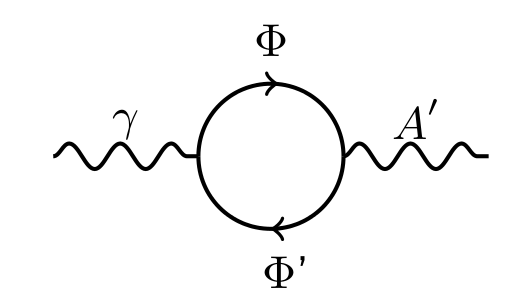
\includegraphics[width=0.5\textwidth]{images/aprime_loop.png}
    \caption{Kinetic mixing of a Standard Model photon with a heavy photon 
    at one-loop through the interaction of massive fields charged under
    the Standard Model hypercharge and dark charge.}
    \label{fig:ap_loop}
\end{figure}
Integrating out the fields generates values of $\epsilon$ on the order of 
\begin{equation}
    \epsilon \sim \frac{g_Yg_D}{16\pi^2}\ln\left(\frac{m_{\Phi}}{m_{\Phi'}} \right)
             \sim 10^{-3} - 10^{-1} 
\end{equation}
where $g_Y$ ($g_D$) are the SM hypercharge (dark) coupling and 
$(m_{\Phi}, m_{\Phi'})$ are the masses of the two fields 
\cite{ArkaniHamed:2008qp, Bjorken:2009mm}.  If the theory doesn't contain 
split multiplets charged under both $U(1)_Y$ and $U(1)'$, the mass splittings 
can be generated by additional loops, leading to values of $\epsilon \sim 10^{-6} - 10^{-3}$. 
In some string theory constructions, 
values as small as $\epsilon \sim 10^{-12}$ are expected 
\cite{Goodsell:2010ie,Goodsell:2009xc, Cicoli:2011yh}.

%
% If I have time, I need to add a paragraph explaining how an A' would acquire
% mass.
%

The possibility that a new gauge boson can couple to charged SM particles is 
very appealing.  It may offer one of the few portals to probe a new sector 
composed of light weakly coupled particles and possibly dark matter
(see section 1.2).  Such a coupling can be exploited by current and future
experimental programs in order to measure the properties of
the hidden sector and possibly provide insight into may outstanding physics puzzles.

\section{Motivations for a Heavy Photon from Dark Matter}

Although the existence of dark matter (DM) has been firmly established through its
gravitational interaction \cite{popolo2014}, its exact nature continues to elude
us. An appealing
possibility is that DM inhabits a ``hidden sector'' with its interactions 
mediated by an $A'$.  In turn, the kinetic mixing of the $A'$ with the SM 
photon may provide a portal that would allow the exploration of not only the 
properties of DM but the hidden sector itself.  Furthermore, several recently
observed astrophysical anomalies \cite{pamela2008, ackermann2012, aguilar2013, 
hooper2011, linden2011, abazajian2012, hooper2013, Bulbul:2014sua}
may have a dark matter interpretation if DM
charge under an $A'$.  A summary of those anomalies along with their dark matter
interpretation will be presented here.

\subsection{Cosmic Rays}

Interest in hidden sector models surged in 2008 with the announcement by 
The Payload for Antimatter Matter Exploration and Light-nuclei Astrophysics \\ 
(PAMELA) of an unforeseen rise in the ratio of the cosmic ray (CR) positron flux
to CR electron flux, $e^{+}/(e^{+} + e^{-})$, above 10 GeV \cite{pamela2008}.
The rise was later confirmed by both the 
Fermi Gamma-Ray Space Telescope \cite{ackermann2012} and Alpha Magnetic 
Spectrometer-02 (AMS-02) \cite{aguilar2013} experiments and observed to continue
up to 200 GeV. 

The main source of CR positrons 
was expected to come from the interaction of CR nuclei with the interstellar 
medium (secondary production).  If such a production mechanism was dominant, 
cosmic ray propagation models predicted the fraction would fall with increasing
energy.  The observed rise lead to the speculation of additional sources of 
positrons including pulsars\cite{yin2013, linden2013}.

One attractive scenario that could account for the rise was the annihilation of
DM to leptons ($e^+e^-, \mu^+\mu^-$). In fact, such models where found to fit 
the data fairly well.  However, such models require much 
larger annihilation rates compared to those expected assuming the typical 
thermal cross-section \cite{Cholis:2008hb}
\begin{equation}
    \left \langle \sigma v \right \rangle \simeq 3 \times 10^{-26} \text{cm}^3 \text{s}^{-1}.
\end{equation}

Alternatively, if DM interactions are mediated by a heavy photon, a 
``Sommerfeld enhancement'' of the annihilation cross-section proportional to
$\sigma v \sim 1/v$ can occur \cite{ArkaniHamed:2008qn}. In such scenarios, the
``freeze-out'' cross-section that leads to the currently observed relic
abundance remain unaffected since the velocity of DM in the early universe was
high and the Sommerfeld enhancement had not effectively turned on.  If the 
heavy photons created in the annihilation of DM subsequently decay to leptons
(Fig. \ref{fig:dm_annihilation}), the resulting $e^+e^-$ spectrum could
account for rise.
\begin{figure}[t]
    \centering
    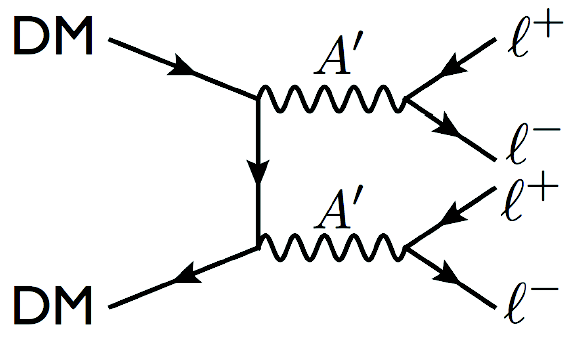
\includegraphics[width=0.5\textwidth]{images/dm_annihilation.png}
    \caption{Dark matter annihilation to a heavy photon which subsequently 
             decays into a pair of leptons.}
    \label{fig:dm_annihilation}
\end{figure}

The most recent measurements of the cosmic microwave background (CMB) have made
it difficult to interpret the positron anomaly as coming from the annihilation
of DM.  
%were to annihilate
%to a heavy photon of mass $\sim$ GeV which subsequently decays to an 
%$e^{+}e^{-}$ 
%the annihilation cross-section of DM at low velocities can be achieved 

%The most recent observations by AMS-02 seem to favor 
%This model became less favorable as higher
%precision measurements of the positron flux became available.  In fact, 
%recent measurements of the cosmic microwave background (CMB) have put very 
%tight constraints on such a scenario.

\subsection{Light Dark Matter}

Recently, an analysis of three years of data collected by the Fermi Large Area
Telescope observed an extended emission in the spectrum of gamma-rays 
originating from the Galactic Center 
\cite{hooper2011, linden2011, abazajian2012, hooper2013}.  Several models have been 
devised to try to explain the emission including the collision of energetic 
protons accelerated by a super-massive black hole \cite{Hooper:2010mq}, 
pulsars \cite{Abazajian:2010zy} and dark matter annihilation to leptons or 
hadron \cite{Hooper:2010mq, Goodenough:2009gk}.  The emission can also
be explained in the context of dark matter annihilating to an $A'$ which 
subsequently decays to SM particles \cite{Hooper:2012cw}.  Such a model assumes
a dark matter candidate of mass $\sim$ 10 GeV annhilating to a heavy photon
with a mass $\sim$ 100 MeV. 

Another anomaly that can be explained in the context of a light dark matter
candidate that couples to a heavy photon is the observance
of a 3.5 keV X-ray line from a 73 galaxy clusters \cite{Bulbul:2014sua}.  
Specifically, the ``eXciting Dark Matter'' model \cite{Finkbeiner:2014sja} 
proposes the existence of a doublet of DM states whose self interactions are 
mediated by a heavy photon. As shown of Figure \ref{fig:dm_self_scat}, a pair
of DM particles upscatter via an $A'$ to produce a pair of excited states, 
$\chi^*\chi^*$. This is immediately followed by the decay 
$\chi^* \rightarrow  \chi\gamma$, producing an X-ray line.
\begin{figure}[t]
    \centering
    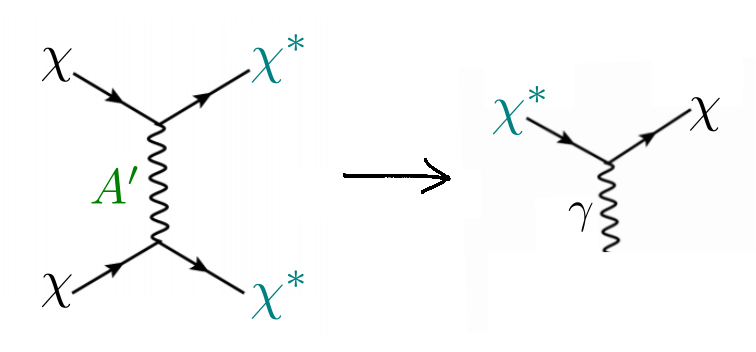
\includegraphics[width=0.9\textwidth]{images/xdm.png}
    \caption{A diagram depicting the self-scattering of dark matter via a heavy
             photon into an excited state. The excited state subsequently decays
             producing an observable X-ray line.}
    \label{fig:dm_self_scat}
\end{figure}


\section{Current Limits on Heavy Photons}
\begin{figure}[ht]
    \centering
    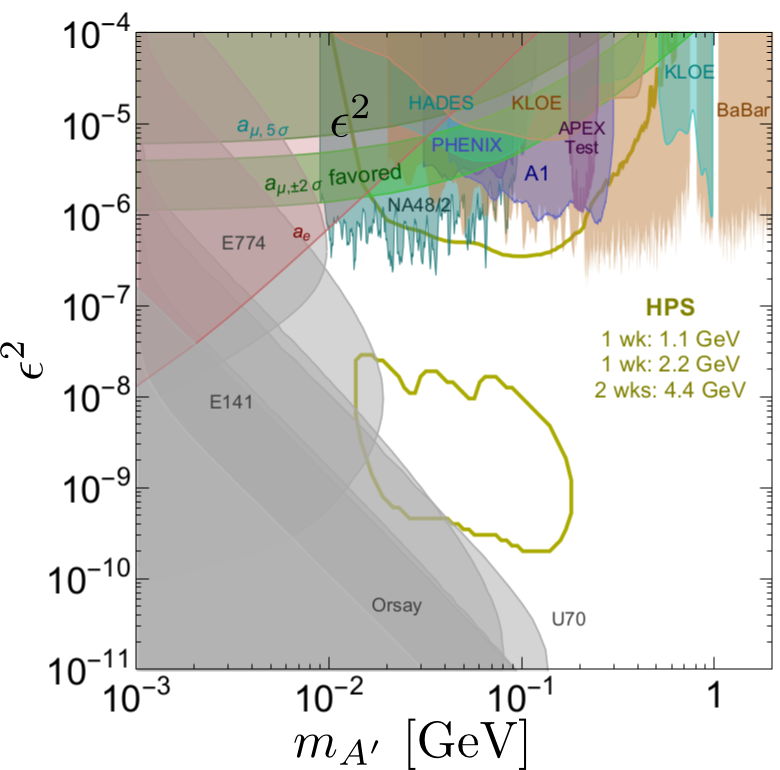
\includegraphics[width=0.9\textwidth]{images/ap_current_limits.png}
    \caption{The estimated 2$\sigma$ reach of the Heavy Photon Search (HPS) 
             experiment along with existing constraints from beam dump  
             \cite{},
             collider \cite{}, 
             and fixed target experiments
             \cite{}.
         The reach calculation assumes HPS running at 1.1 GeV}
    \label{fig:ap_limits}
\end{figure}

\subsection{Electron Beam Dump Experiments}

Electron beam dump experiments make use of a high intensity beam ``dumped'' onto
a thick ($\sim$ cm) target to produce highly boosted heavy photons through a 
process analogous to photon bremsstrahlung.  In order to suppress the large
SM backgrounds produced at the target, a shield of thickness $\sim$ cm - m
is placed immediately downstream, and in front of the detector.  Since the 
heavy photons weakly interact with SM particles, sufficiently long lived 
heavy photons will traverse the shield before reaching an open space upstream
of a detector.  The decay products of heavy photons decaying in this region 
will travel unimpeded until detected.
The thickness of the target and shield in combination with a high luminosity
beam allow such experiments to be sensitive to heavy photons with small 
couplings which tend to travel considerable distances before decaying. Such 
experiments tend to be sensitive to heavy photons with 
$10^{-7} \le \epsilon 10^{-3}$  of masses on the order of 100 MeV. 

% What backgrounds are these experiments concerned with?
% What is the shield made of?

Several electron beam dump experiments were devised over the last several decades with
the intention of searching for axions \footnote{Axions are particles postulated 
by Peccei-Quinn in the last 70's in order to the strong CP problem}.  These 
included E137 \cite{Bjorken:1988as}
and E141 \cite{riordan1987} conducted at SLAC National Accelerator Laboratory,
E774 \cite{bross1991} at Fermi National Accelerator Laboratory, and experiments at 
KEK \cite{konaka1986} in Japan and Orsay \cite{davier1989} in France. 
%The setup of each of the experiments is summarized on Table \ref{}. 
The results from each of these experiments have been reinterpreted in the 
context of a search for a heavy photon and used to set limits on the coupling
strength $\epsilon$ \cite{Bjorken:2009mm, andreas2012}.  The resulting limits are 
shown on Fig. \ref{fig:ap_limits}.

\subsection{Proton Beam Dump Experiments}

Proton beam dump experiments can also be used to search for heavy photons
through either the decay of mesons produced at the target or proton
bremsstrahlung.  The data collected by one such experiment that used the U70
accelerator at IHEP Serpukhov, was originally devised to search for both axions
and a light Higgs boson \cite{Blumlein:1990ay, Blumlein:1991xh}.  The data was 
re-analyzed and a search for an $A'$ was conducted
using the $\pi_0 \rightarrow A'\gamma$ decay channel and proton bremsstrahlung
\cite{johannes2011, johannes2014}. The resulting limits are shown on Fig. 
\ref{fig:ap_limits}.

\subsection{Electron-Positron Colliders}

The past decade saw the operation of several high-luminosity $e^+e^-$ colliders 
that were able to collect a lot of data at different center-of-mass energies.
These include KLOE running at the the DA$\Phi$NE $\phi$ factory and BaBar, 
at the PEP-II B-Factory. Searches at BaBar were performed using the channel 
$e^+e^- \rightarrow A' \gamma (A' \rightarrow \mu^+\mu^-)$ 
\cite{Reece:2009un, Aubert:2009cp}.  KLOE 
searched for heavy photons in the decays of the $\phi$ meson.  Specifically, 
the channel $\phi \rightarrow \eta A' (A' \rightarrow e^+e^-)$ was used to
set limits on the coupling strength of the $A'$ 
\cite{Babusci:2012cr, Archilli:2011zc}.
The limits set by both BaBar and KLOE are shown on Fig. \ref{fig:ap_limits}.

\subsection{Electron Fixed Target Experiments}

\section{The Heavy Photon Search Experiment}

